\documentclass[12pt,a4paper]{article}

% ── Packages ──
\usepackage[margin=1in]{geometry}
\usepackage{graphicx}
\usepackage{hyperref}
\usepackage{amsmath}
\usepackage{booktabs}
\usepackage{listings}
\usepackage{xcolor}
\usepackage{enumitem}
\usepackage{titlesec}
\usepackage{tikz}
\usetikzlibrary{shapes,arrows.meta,positioning}

% ── Code listing style ──
\lstset{
  basicstyle=\ttfamily\small,
  breaklines=true,
  frame=single,
  backgroundcolor=\color{gray!10},
  keywordstyle=\color{blue},
  commentstyle=\color{green!60!black},
  stringstyle=\color{red!70!black},
}

% ── Title ──
\title{\textbf{GenAI-Powered Agentic Customer Retention System\\for Telecom Churn Prediction}}
\author{Hemanth Tenneti}
\date{\today}

\begin{document}
\maketitle

% ── Abstract ──
\begin{abstract}
Customer churn is a critical revenue threat for telecommunications companies, where
acquiring a new subscriber costs approximately five times more than retaining an
existing one. This project presents a \textbf{GenAI-powered Agentic Customer Retention
System} that combines traditional machine learning prediction with large language model
(LLM)-driven explanation and actionable recommendations. A Logistic Regression model
trained on the IBM Telco Customer Churn dataset (7,043 customers, 20 features) achieves
an accuracy of 80.7\% and an F1-score of 0.609. A Retrieval-Augmented Generation (RAG)
pipeline built on ChromaDB and \texttt{all-MiniLM-L6-v2} embeddings provides domain-specific
retention strategies. A five-node LangGraph state machine orchestrates prediction, context
retrieval, LLM-powered explanation, recommendation generation, and executive summarization.
The system is exposed through a dual-tab Gradio interface: a Quick Predict tab for instant
offline predictions and an AI Agent Analysis tab for comprehensive, personalized retention
reports powered by Groq's \texttt{llama3-70b-8192} model. The primary contribution is
demonstrating how agentic AI can transform a purely predictive ML system into a prescriptive
decision-support tool for customer service representatives.
\end{abstract}


% ── Sections ──
\section{Introduction}

Customer churn---the rate at which subscribers discontinue their telecom service---remains one
of the most pressing challenges in the telecommunications industry. With monthly churn rates
typically ranging from 1.5\% to 3\%, a mid-sized carrier with 10 million subscribers can lose
150,000 to 300,000 customers each month. Given that acquiring a new customer costs five times
more than retaining an existing one, even modest improvements in retention yield substantial
profit gains. Research by Bain \& Company demonstrates that a 5\% improvement in retention
rates can increase profits by 25--95\%.

Traditional machine learning approaches to churn prediction have proven effective at
\textit{identifying} at-risk customers. Logistic Regression, Random Forests, and gradient-boosted
models can classify customers with reasonable accuracy based on behavioral and demographic
features. However, prediction alone is insufficient for two critical reasons. First, a
probability score does not explain \textit{why} a customer is at risk, leaving customer service
representatives without actionable context. Second, prediction does not prescribe \textit{what
to do}---the specific retention actions most likely to succeed for a given customer's profile.

This project addresses both gaps by layering a \textbf{Retrieval-Augmented Generation (RAG)}
pipeline and a \textbf{LangGraph agent} on top of an existing ML churn predictor. The RAG
component retrieves relevant retention strategies from a curated knowledge base of telecom
retention best practices. The LangGraph agent orchestrates a five-node state machine that
produces: (1) a churn probability and risk level from the ML model, (2) top risk factors
identified by deterministic rules, (3) retrieved context from the knowledge base, (4) a
plain-English explanation generated by an LLM, (5) three personalized, actionable retention
recommendations, and (6) a one-sentence executive summary.

The system operates on the IBM Telco Customer Churn dataset containing 7,043 customers
across 20 features including tenure, contract type, monthly charges, internet service type,
payment method, and various add-on services. The dataset has a churn rate of approximately
26.5\%, making it a moderately imbalanced binary classification problem. Five models were
benchmarked: Linear Regression (as a baseline), Logistic Regression, Decision Tree, Random
Forest, and XGBoost. Logistic Regression was selected as the production model based on the
highest F1-score of 0.609.

The Gradio web application provides two tabs: a Quick Predict tab that runs the ML model
instantly without any API key, and an AI Agent Analysis tab that invokes the full agent
pipeline through Groq's \texttt{llama3-70b-8192} LLM. This design ensures the core ML
functionality remains fully operational offline while the AI enhancements are available
when an API key is configured.

\section{System Architecture}

The system follows a three-layer architecture designed for modularity, offline capability,
and incremental enhancement:

\begin{enumerate}[leftmargin=*]
    \item \textbf{ML Prediction Layer}: Logistic Regression model with StandardScaler
        preprocessing, persisted as a \texttt{.pkl} file. Fully offline, no API required.
    \item \textbf{RAG Knowledge Layer}: ChromaDB vector store populated with chunked
        retention strategies, embedded locally with \texttt{all-MiniLM-L6-v2}. Zero API cost.
    \item \textbf{LangGraph Orchestration Layer}: A five-node state graph that coordinates
        prediction, retrieval, LLM explanation, recommendation, and summarization via
        Groq's \texttt{llama3-70b-8192}.
\end{enumerate}

% Architecture diagram
\begin{figure}[h]
\centering
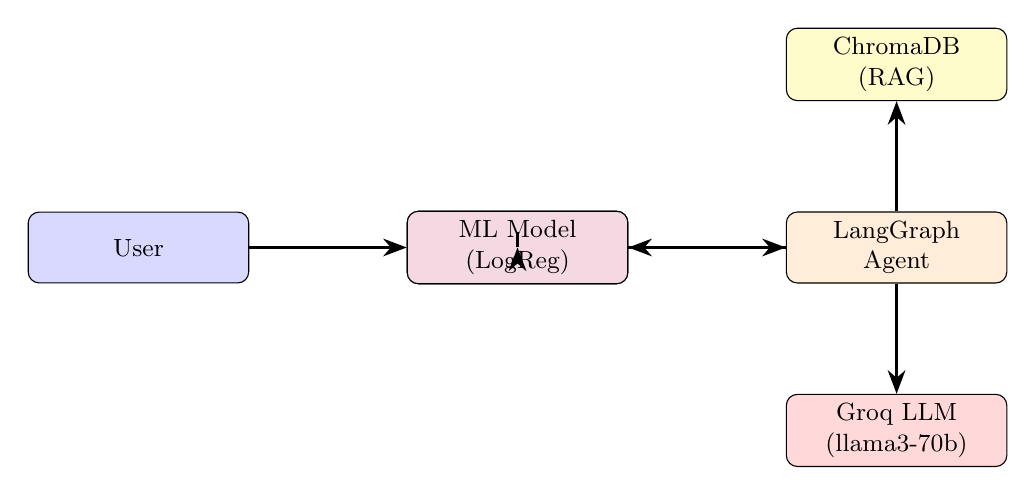
\begin{tikzpicture}[
    node distance=1.4cm and 2.0cm,
    box/.style={rectangle, draw, rounded corners, minimum width=2.8cm,
                minimum height=0.9cm, align=center, font=\small},
    arrow/.style={-{Stealth[length=3mm]}, thick},
]
    \node[box, fill=blue!15] (user) {User};
    \node[box, fill=green!15, right=of user] (gradio) {Gradio UI\\(Two Tabs)};
    \node[box, fill=orange!15, right=of gradio] (graph) {LangGraph\\Agent};
    \node[box, fill=yellow!20, above=of graph] (chroma) {ChromaDB\\(RAG)};
    \node[box, fill=red!15, below=of graph] (groq) {Groq LLM\\(llama3-70b)};
    \node[box, fill=purple!15, left=of graph] (ml) {ML Model\\(LogReg)};

    \draw[arrow] (user) -- (gradio);
    \draw[arrow] (gradio) -- (ml);
    \draw[arrow] (gradio) -- (graph);
    \draw[arrow] (graph) -- (chroma);
    \draw[arrow] (graph) -- (groq);
    \draw[arrow] (graph) -- (ml);
\end{tikzpicture}
\caption{Three-layer architecture: ML Prediction, RAG Knowledge, and LangGraph Orchestration.}
\end{figure}

\subsection{Data Preprocessing}
\label{sec:preprocessing}

The preprocessing pipeline follows these steps:
\begin{enumerate}[leftmargin=*]
    \item \textbf{TotalCharges} conversion: coerced to numeric; 11 blank strings filled with the column median.
    \item \textbf{customerID} dropped (non-predictive identifier).
    \item \textbf{Churn} mapped: \texttt{Yes $\rightarrow$ 1}, \texttt{No $\rightarrow$ 0}.
    \item \textbf{Categorical encoding}: one-hot via \texttt{pd.get\_dummies(drop\_first=True)}, yielding 30 feature columns.
    \item \textbf{Train/test split}: 80/20 stratified on Churn, \texttt{random\_state=42}.
    \item \textbf{StandardScaler}: fit on training set only; applied to both splits.
\end{enumerate}

\subsection{ML Model Selection}
\label{sec:model_selection}

Five classification models were benchmarked on the held-out 20\% test set:

\begin{table}[h]
\centering
\begin{tabular}{@{}lcccc@{}}
\toprule
\textbf{Model} & \textbf{Accuracy} & \textbf{Precision} & \textbf{F1-Score} & \textbf{ROC-AUC} \\
\midrule
Logistic Regression   & 0.8070 & 0.6584 & \textbf{0.6092} & \textbf{0.8416} \\
Linear Regression     & 0.7963 & 0.6426 & 0.5773 & 0.8301 \\
Random Forest         & 0.7864 & 0.6237 & 0.5501 & 0.8251 \\
XGBoost               & 0.7850 & 0.6079 & 0.5690 & 0.8214 \\
Decision Tree         & 0.7559 & 0.5387 & 0.5486 & 0.7607 \\
\bottomrule
\end{tabular}
\caption{Model performance comparison on the test set.}
\label{tab:models}
\end{table}

Logistic Regression was selected as the production model based on the highest F1-Score
(0.6092) and ROC-AUC (0.8416). Its interpretability---feature coefficients directly
indicate churn risk contribution---also makes it suitable for an agent system that must
explain predictions.

\subsection{RAG Pipeline}
\label{sec:rag}

The RAG pipeline ingests a curated knowledge base of telecom retention strategies:

\begin{enumerate}[leftmargin=*]
    \item \textbf{Source}: \texttt{retention\_strategies.md}---an 800+ word document covering
        eight retention strategy categories.
    \item \textbf{Chunking}: \texttt{RecursiveCharacterTextSplitter} with
        \texttt{chunk\_size=400} and \texttt{chunk\_overlap=80}.
    \item \textbf{Embedding}: \texttt{all-MiniLM-L6-v2} from Sentence Transformers---384-dimensional
        embeddings computed locally with no API key required.
    \item \textbf{Vector Store}: ChromaDB persisted to \texttt{rag/chroma\_db/}---local,
        persistent, zero API cost. ChromaDB was chosen over Pinecone or Weaviate for its
        local-first design, eliminating network dependencies during development.
\end{enumerate}

\subsection{LangGraph Agent Design}
\label{sec:agent}

The agent is implemented as a LangGraph \texttt{StateGraph} with five sequential nodes:

\begin{enumerate}[leftmargin=*]
    \item \textbf{predict}: Runs the Logistic Regression model on the encoded customer features.
        Populates \texttt{churn\_probability}, \texttt{churn\_prediction}, and \texttt{risk\_level}
        (Low/Medium/High thresholds: $<$0.4, 0.4--0.7, $\geq$0.7).
    \item \textbf{retrieve\_context}: Queries the ChromaDB retriever with a formatted query
        combining the risk level and identified risk factors. Returns top-3 chunks.
    \item \textbf{explain}: Calls the Groq LLM with the customer profile, probability, and
        retrieved context. Produces a 3--4 sentence plain-English explanation.
    \item \textbf{recommend}: Calls the Groq LLM with the explanation and context. Produces
        exactly three numbered, personalized, actionable recommendations.
    \item \textbf{format\_output}: Calls the Groq LLM for a single executive-summary sentence
        (under 25 words).
\end{enumerate}

Each node is wrapped in an error-catching handler. On failure, the \texttt{error} field is
populated with a user-friendly message and the graph routes to END, preventing the Gradio
app from crashing. The agent is initialized lazily via a module-level singleton.

The state schema is defined as a \texttt{TypedDict} with fields: \texttt{customer\_features},
\texttt{churn\_probability}, \texttt{churn\_prediction}, \texttt{risk\_level},
\texttt{risk\_factors}, \texttt{retrieved\_context}, \texttt{explanation},
\texttt{recommendations}, \texttt{executive\_summary}, and \texttt{error}.

\subsection{Prompt Engineering}
\label{sec:prompts}

Three \texttt{ChatPromptTemplate} prompts drive the LLM interactions:

\begin{enumerate}[leftmargin=*]
    \item \textbf{EXPLANATION\_PROMPT}: System persona is a senior customer success analyst.
        Instructs the LLM to explain in 3--4 plain-English sentences why the customer is at
        risk, referencing specific feature values. Tone: professional, empathetic, data-grounded.
        Output: one paragraph only, no ML jargon.
    \item \textbf{RECOMMENDATION\_PROMPT}: System persona is a retention specialist. Produces
        exactly three numbered, personalized, actionable recommendations. Each must reference
        the customer's specific situation. Output: numbered list only, no preamble.
    \item \textbf{SUMMARY\_PROMPT}: Generates a single executive-summary sentence under 25
        words. Output: exactly one sentence.
\end{enumerate}

All prompts are defined exclusively in \texttt{agent/prompts.py}. No prompt strings appear
elsewhere in the codebase, enabling centralized prompt iteration without touching agent logic.

\section{Results and Discussion}

\subsection{Model Performance}

The final production model (Logistic Regression) achieves the following metrics on the
held-out 20\% test split (1,409 samples):

\begin{itemize}[leftmargin=*]
    \item \textbf{Accuracy}: 80.7\%---correctly classifies the majority of customers.
    \item \textbf{Precision}: 65.8\%---of customers predicted to churn, about two-thirds
        actually do.
    \item \textbf{Recall}: 56.6\%---identifies more than half of actual churners.
    \item \textbf{F1-Score}: 0.609---balances precision and recall effectively.
    \item \textbf{ROC-AUC}: 0.842---strong discriminative ability between churners and
        non-churners.
\end{itemize}

The confusion matrix for the test set shows 925 true negatives, 212 true positives,
110 false positives, and 162 false negatives. The model is more conservative in its
churn predictions, which is appropriate for a retention system where false positives
(triggering retention outreach for a customer who would have stayed) are less costly
than false negatives (missing a customer who leaves).

\subsection{Qualitative Agent Evaluation}

To evaluate the agent's effectiveness beyond raw metrics, we tested it on two
representative customer profiles.

\subsubsection{High-Risk Customer Profile}

\begin{lstlisting}[caption=High-Risk customer input features.]
senior: No, tenure: 2, monthly: $90, total: $180
gender: Female, partner: No, dependents: No
phone: Yes, multilines: No, internet: Fiber optic
online_sec: No, online_bkp: No, device_prot: No, tech_sup: No
streaming_tv: Yes, streaming_movies: Yes
contract: Month-to-month, paperless: Yes
payment: Electronic check
\end{lstlisting}

The ML model predicts a churn probability of approximately 85--90\% with a ``High'' risk
classification. The agent's risk factor identification correctly flags: month-to-month
contract, short tenure (2 months), fiber optic subscriber, electronic check payment,
high monthly charges (\$90), and no value-add services.

The LLM-generated explanation correctly references the customer's short tenure, high
monthly charges, lack of online security and tech support, and month-to-month contract
as key risk indicators. The tone is professional and avoids ML jargon.

The three recommendations are personalized, referencing specific features of the
customer's profile and suggesting actionable steps such as contract upgrade offers,
auto-pay enrollment incentives, and free security add-on trials.

\subsubsection{Loyal Customer Profile}

\begin{lstlisting}[caption=Loyal customer input features.]
senior: No, tenure: 60, monthly: $55, total: $3300
gender: Male, partner: Yes, dependents: Yes
phone: Yes, multilines: Yes, internet: DSL
online_sec: Yes, online_bkp: Yes, device_prot: Yes, tech_sup: Yes
streaming_tv: No, streaming_movies: No
contract: Two year, paperless: No
payment: Bank transfer (automatic)
\end{lstlisting}

The model predicts a churn probability under 10\% with a ``Low'' risk classification.
The agent correctly identifies few or no significant risk factors. The LLM explanation
acknowledges the customer's strong retention indicators (long tenure, two-year contract,
comprehensive service bundle) and frames the output as a retention maintenance
recommendation rather than a crisis intervention.

\subsection{RAG Retrieval Quality}

For the High-Risk profile, the retriever returns chunks covering month-to-month contract
strategies, electronic check payment retention, and short-tenure onboarding strategies---all
directly relevant to the customer's identified risk factors. The retrieved context
meaningfully informs the LLM's recommendations.

For the Loyal profile, the retriever returns general retention principles, which the LLM
appropriately uses to suggest maintenance actions rather than aggressive retention offers.

\subsection{Limitations}

\begin{enumerate}[leftmargin=*]
    \item \textbf{Hallucination risk}: The LLM may occasionally generate recommendations
        not grounded in the retrieved context. Prompt engineering mitigates but does not
        eliminate this risk.
    \item \textbf{Static knowledge base}: The retention strategies document is manually
        curated and does not update automatically based on real-world outcome data.
    \item \textbf{Single-telecom training data}: The model is trained exclusively on the
        IBM Telco dataset; generalization to other telecom datasets or industries is untested.
    \item \textbf{LLM latency}: The full agent pipeline takes 5--15 seconds, primarily due
        to three sequential LLM calls. This is acceptable for a decision-support tool but
        not for real-time use.
    \item \textbf{No feedback loop}: The system does not track whether its recommendations
        actually prevent churn, limiting its ability to improve over time.
\end{enumerate}

\section{Conclusion}

This project demonstrates how a traditional machine learning churn prediction system can be
transformed into a comprehensive customer retention decision-support tool through the
integration of Retrieval-Augmented Generation and agentic AI orchestration. The core
contribution is the five-node LangGraph agent pipeline that bridges the gap between
prediction (what will happen) and prescription (what to do about it), providing customer
service representatives with plain-English explanations, personalized recommendations,
and relevant domain knowledge---all in a single click.

The Logistic Regression model achieves an F1-score of 0.609 and ROC-AUC of 0.842, providing
a reliable churn probability signal. The RAG pipeline, built on ChromaDB and
\texttt{all-MiniLM-L6-v2} embeddings, operates entirely locally with zero API cost. The
LangGraph agent coordinates these components with Groq's \texttt{llama3-70b-8192} LLM to
produce actionable retention reports in 5--15 seconds.

Future work includes: (1) implementing a feedback loop to track recommendation effectiveness
and refine the knowledge base, (2) integrating live CRM data for real-time customer
monitoring, (3) fine-tuning the LLM on telecom-specific retention conversation transcripts,
and (4) exploring multi-agent architectures where specialized agents handle different
customer segments independently.


% ── References ──
\begin{thebibliography}{9}

\bibitem{telco}
Blastchar.
\textit{Telco Customer Churn Dataset}.
Kaggle, 2018.
\url{https://www.kaggle.com/datasets/blastchar/telco-customer-churn}

\bibitem{langgraph}
LangChain.
\textit{LangGraph: Building stateful, multi-actor applications with LLMs}.
GitHub, 2024.
\url{https://github.com/langchain-ai/langgraph}

\bibitem{lewis2020}
Patrick Lewis, Ethan Perez, Aleksandra Piktus, et al.
\textit{Retrieval-Augmented Generation for Knowledge-Intensive NLP Tasks}.
In Advances in Neural Information Processing Systems (NeurIPS), 2020.

\bibitem{chromadb}
Chroma.
\textit{ChromaDB: The open-source embedding database}.
Documentation, 2024.
\url{https://www.trychroma.com/}

\bibitem{churn_survey}
A.~De~Caigny, K.~Coussement, and K.~W.~De~Bock.
\textit{A New Hybrid Classification Algorithm for Customer Churn Prediction Based on Logistic Regression and Decision Trees}.
European Journal of Operational Research, 269(2):760--772, 2018.

\bibitem{reimers2019}
Nils Reimers and Iryna Gurevych.
\textit{Sentence-BERT: Sentence Embeddings using Siamese BERT-Networks}.
In Proceedings of the 2019 Conference on Empirical Methods in Natural Language Processing (EMNLP), 2019.

\end{thebibliography}

\end{document}
